\documentclass[12pt]{article}

\usepackage{float}
\usepackage{amsmath}
\usepackage{amsfonts}
\usepackage{gensymb}
\usepackage{tikz}

\begin{document}
\title{AP Physics C: Circular Motion}
\author{Raja Williams}
\date{December 2023}
\maketitle

\section{Objective}
The purpose of the Circular Motion lab was to determine the acceleration due to
gravity on a plane that is flying around in a circle.

\section{Procedure}

After the plane is launched, the system for the following procedures can be seen
in Figure \ref{fig:overview}.

\begin{figure}[h]
    \centering
    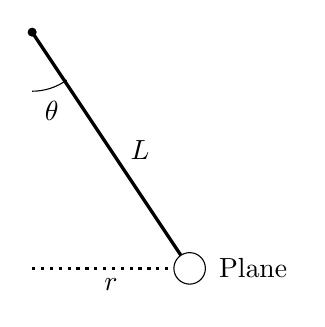
\begin{tikzpicture}
        \draw (0,-0.75) arc (-90:-54.217:0.75);
        \draw[very thick, dotted] (0,-3) -- (2,-3);
        \draw[very thick] (0,0) -- (2,-3);
        \draw[fill=black] (0,0) circle [radius=0.05];
        \draw[fill=white] (2,-3) circle [radius=0.2];
        \draw (1.125,-1.5) node[anchor=west] {$L$};
        \draw (0.25,-0.75) node[anchor=north] {$\theta$};
        \draw (2.25,-3) node[anchor=west] {Plane};
        \draw (1,-3) node[anchor=north] {$r$};
    \end{tikzpicture}
    \caption{Diagram of lab setup.}
    \label{fig:overview}
\end{figure}

Collect any required data to determine $\overline{r}$:
\begin{enumerate}
    \item Set up the lab as detailed in the Lab Procedure.
    \item Grab and stop the plane while it is still flying.
    \item Place a meter stick directly under the magnetic hook to establish a
        origin of rotation for the plane.
    \item Using a meter stick, measure $r$ by measuring the distance from the
        origin of rotation to the plane.
    \item Repeat Steps 1-4 around five times.
    \item Calculate $\overline{r}$ with collected data.
\end{enumerate}

Collect any required data to determine $\overline{\omega}$:
\begin{enumerate}
    \item Set up the lab as detailed in the Lab Procedure.
    \item Start and hold a timer in front of a slow-motion capable camera.
    \item Begin recording the rotation of the plane in slow-motion. Ensure timer
        is in frame.
    \item End recording after around 5-10 revolutions of the plane.
    \item Find period with recorded footage by analyzing time between
        revolutions using the timer in the footage.
    \item Calculate $\overline{T}$ with collected data.
    \item Calculate $\overline{\omega}$ with $\overline{T}$.
\end{enumerate}

\section{Observations and Data}

We found that $L$ equals 1 m.

To calculate $\overline{r}$, we captured five data points, shown in Figure
\ref{fig:r_data}.

\begin{figure}[H]
    \centering
    \begin{tabular}{| r | l |}
        \hline
        Trial & $r$ \\ \hline
        1 & 70 cm \\
        2 & 69 cm \\
        3 & 69 cm \\
        4 & 68 cm \\
        5 & 66 cm \\
        \hline
    \end{tabular}
    \caption{Table of the data collected for $\overline{r}$.}
    \label{fig:r_data}
\end{figure}

To measure $\overline{T}$, we captured an indeterminate amount of data
points. This data is unavailable due to unforeseen circumstances.

\section{Analysis}

Using the data for $r$, we can calculate that $\overline{r}$ equals $68.4 \pm
0.5$ cm. As well, using the data for $T$, we can calculate that $\overline{T}$
equals $1.81 \pm 0.1$ s. Using T, we can then find $\overline{\omega}$.

\begin{align*}
    \begin{split}
        \frac{2 \pi}{\overline{\omega}} &= \overline{T} \\
        \frac{\overline{\omega}}{2 \pi} &= \frac{1}{\overline{T}} \\
        \overline{\omega} &= \frac{2 \pi}{\overline{T}} 
    \end{split}
\end{align*}

Using $\overline{T}$, we can calculate that $\overline{\omega}$ equals 3.47
rad/s.

To calculate the $F_g$, and thus the acceleration due to gravity, we must first
make clear the mechanics that the plane is undergoing. As shown in
\ref{fig:fbd}, the $F_t$ is angled and, in the diagram, is comprised of two
components. Since the plane is not falling, we know that $F_{t_z}$ must be equal
to $F_g$. As well, we also know that $F_{t_r}$ must equal $m \cdot a_c$, where
$m$ is the mass of the plane and $a_c$ is the centripetal acceleration.

\begin{figure}[h]
    \centering
    \begin{tikzpicture}
        \draw[fill=black] (0,0) circle [radius=0.075];
        \draw[->] (-3,0) -- (3,0) node[right] {$r$};
        \draw[->] (0,-3) -- (0,3) node[above] {$z$};
        \draw[dotted,thick] (1,2) -- (0,2) node[left] {$F_{t_r}$};
        \draw[dotted,thick] (1,2) -- (1,0) node[below] {$F_{t_z}$};
        \draw[->,ultra thick] (0,0) -- (0,-2) node[right] {$F_g$};
        \draw[->,ultra thick] (0,0) -- (1,2) node[above] {$F_t$};
        \draw (0.25,0.75) node[anchor=south] {$\theta$};
        \draw (0,0.75) arc (90:63.435:0.75);
    \end{tikzpicture}
    \caption{Free body diagram of the plane in flight.}
    \label{fig:fbd}
\end{figure} 

So, utilizing the fact that we know $F_{t_r}$, we can solve for $F_t$:

\begin{align*}
    \begin{split}
        F_{t_r} &= m a_c \\ 
        F_{t_r} &= m w^2 r \\
        F_{t_r} &= m w^2 L \sin \theta \\
        F_t &= m w^2 L
    \end{split}
\end{align*}

With $F_t$, we can now solve for $F_g$, and then $g$.

\begin{align*}
    \begin{split}
        F_{t_y} &= F_g \\ 
        m w^2 L \cos \theta &= F_g \\
        m w^2 L \cos \theta &= mg \\
        w^2 L \cos \theta &= g
    \end{split}
\end{align*}

With $\overline{r}$, we can calculate $\theta$ to be about 0.753 rad. With that,
we can calculate $g$ to be about 8.79 m/s\textsuperscript{2}.

\section{Conclusion}

With a $g$ of 8.79 m/s\textsuperscript{2}, the percent error of our prediction
is -10.306\%. By far the factor that introduced the most error would be the
misalignment of the origin of rotation meter stick while trying to measure $r$.
Due to human error, the origin of rotation meter stick was not perfectly aligned
with the magnetic hook on the ceiling, nor did it point perfectly down in the
direction of gravity. This would introduce error as the $r$ values measured
could be misaligned relative to the axis of rotation.

\end{document}

